\chapter{Preparation of Glazes}
Glazes should be prepared in a systematic manner in order to prevent mistakes. 
Most problems with glazes come from simple things, like incorrect weighing, 
mistakes in identifying raw materials or not sieving the glaze correctly.

Glaze mistakes are expensive, as they can result in the loss of an entire 
kilnload. For this reason, it is important to have the right person in charge 
of making glazes--cleanliness, orderliness, careful record-keeping, and 
reliability are required.

Most small producers do not need a large variety of glazes -in fact, many use 
only one or two standard glazes and achieve variety by changing the colors, 
doubleglazing or using engobe decoration.

Designing a glaze is somewhat like choosing a paint in the paint store. First 
of all, you must decide if you want a glossy or matt surface, transparent or 
opaque. Then you can add different colors.
%-------------------------------------------------------------------------------
\subsection*{Base Glaze}
The base glaze is simply the combination of materials that melts at the desired 
temperature. It is either transparent or opaque, matt, semimatt, glossy etc. 
without any particular color.
%-------------------------------------------------------------------------------
\subsection*{Glaze Additions}
These are usually coloring oxides that are added to the glaze. In Nepal a glaze 
supplying system serving small producers was established. A base glaze was 
supplied in 5kg bags and 8 different colors were supplied in small bags that 
produced standard colors when added to 5 kg base glaze. The small bags contain 
coloring oxides mixed with a small amount of base glaze so the colors disperse 
more easily in the base glaze.
%-------------------------------------------------------------------------------
\section{Raw Materials Requirements}
Raw materials need to be as reliable as possible and always ground to the same 
mesh. If obtained from a glaze supplier, the materials are usually ground to at 
least 100 mesh. Because materials that are finely ground melt more easily, some 
ingredients may be as fine as 400 mesh. This is particularly true of 
quartz--200-mesh quartz will produce a different result than 400-mesh quartz.

When you get new raw materials, they always should be tested before using them 
in production. The best way is to try them in a standard glaze that you know 
well and to compare the results with the known glaze.
%-------------------------------------------------------------------------------
\section{Grinding Glaze Materials}
%-------------------------------------------------------------------------------
\subsection{Coarse Materials}
There are several steps in grinding glaze materials. Since many of them 
(feldspar, quartz, limestone) come as rocks, they first need to be reduced to 
pebble size. Feldspar and quartz rocks are first calcined to make them soft 
enough to crush. Calcining means firing to just above 600\degree C. This can be 
done 
in the cold spots of a biscuit firing or for large productions in a special 
kiln. Crushing of small amounts can be done with a hammer (use eye protection), 
and large amounts are usually done in a jaw crusher.
%-------------------------------------------------------------------------------
\subsection{Ball Milling}
\subsubsection{Ball Mill Operation}
Ball mills are used for fine grinding of ceramic materials. The material has to 
be reduced to sand size (2 mm or less) before grinding in a ball mill.

Some typical uses of ball mills are:
%-------------------------------------------------------------------------------
\begin{itemize}
\item grinding clay that does not easily slake
\item preparation of casting slips
\item grinding of body additions like feldspar, quartz and glass powder
\item grinding of frit granules grinding of glazes
\item grinding of engobes and terra sigillata
\item preparing color pigments for glaze, engobes or bodies.
\end{itemize}
%-------------------------------------------------------------------------------
There are two main types of mills:
%-------------------------------------------------------------------------------
\begin{itemize}
  \item Large mills with an axle system are called ball mills.
  \item Small mills are called pot mills or jar mills.
  
  These are usually small (up to 5--liter) porcelain jars or plastic jars, 
  which 
  rotate on two rubber-covered rollers.
\end{itemize}
%-------------------------------------------------------------------------------
\subsubsection{Conical ball mill}
For large production conical ball mills are used. Various sizes of pebbles are 
used and the material is fed from one end and discharged at the other. 
Variation of the centrifugal force caused by a conical 30\degree slope at the 
discharge side classifies both pebbles and material so only fine material is 
discharged.
%-------------------------------------------------------------------------------
\subsubsection{Vibro energy mill}
This is a new type of grinding machine consisting of cylindric grinding chamber 
suspended on springs and vibrated at high frequency with the help of an 
excentric mounted on an electric motor. The chamber is completely packed with 
very hard small cylinders between which the material is filled. The vibrations 
make the small cylinders grind against each other and the material to be 
ground. The vibrating mill is better at ultrafine grinding and is more 
energy-efficient than ball mills.
%-------------------------------------------------------------------------------
\subsubsection{Lining}
The grinding action takes place between the pebbles, and not between the 
pebbles and lining. Therefore a ball mill with a steel drum can work without a 
lining (except for white body, where rust particles will cause discoloration). 
Pebbles constantly falling on a steel drum make a lot of noise. A lining will 
reduce the noise and at the same time prolong the life of the steel. 
Traditionally, linings are made of porcelain or stoneware bricks set in a 
cement mortar, using high alumina cement and coarse silica sand. Common cement 
can be used if necessary but may cause pinhole problems in glazes. The bricks 
should be dense and vitreous. A porcelain body for lining bricks and pebbles 
(fire to 1250\degree C or higher) is shown in table~\ref{tab:liningbody}.

One type of brick is made concave to fit the curve of the drum and another type 
is made for the end walls of the drum.

Linings can be made from granite, quartzite or similar hard rocks (not 
limestone or marble). They are cut to shape and set in a high alumina cement 
mortar. They last far longer than porcelain bricks. Stoneware bricks can be 
used for the end walls, which are worn out more slowly.

Instead of a hard lining, thick rubber sheet glued to the inside makes a very 
long-lasting and quiet lining.
%------------------------------------------------------------------------------
\begin{center}
          \renewcommand{\arraystretch}{1.5}
  \begin{table}\centering
    \begin{tabular}{|c|c|}\hline
      \textbf{Ingredient}&\textbf{Percent}\\\hline\hline
      %------------------------------------------------------------------------------
      China clay&40\%\\\hline
      %------------------------------------------------------------------------------
      Quartz&25\%\\\hline
      %------------------------------------------------------------------------------
      Feldspar&30\%\\\hline
      %------------------------------------------------------------------------------
      Ball clay&5\%\\\hline
    \end{tabular}
    \caption{A porcelain body for lining bricks and pebbles.}
    \label{tab:liningbody}
  \end{table}
\end{center}
%------------------------------------------------------------------------------
\subsubsection{Pebbles}
Pebbles or balls can be made from vitreous clay bodies. However, it is often 
cheaper to collect stones of granite, quartz or quartzite along riverbeds. 
Flint, a variety of quartz, is excellent for pebbles. The hardness is tested 
with a penknife to make sure it is above 5.5 (see Mohs' scale, 
table~\ref{tab:mohs}). Pebbles of limestone are not satisfactory, as they 
contaminate the glaze. The shape should not be flat or elongated but spherical. 
(Cylinders of equal diameter and length are sometimes used to obtain particles 
with less variation in particle size.) Size should be between 2.5 and 5 cm in 
diameter.

Pebbles wear out, so occasionally take out all the pebbles for inspection. 
Those that are broken or flat should be discarded. In large mills, pebbles are 
removed when they are less than 2--3 cm. In small mills pebbles smaller than 
1.5--2 cm are discarded.

As the pebbles grind down, they contribute a small amount of material to the 
glaze. Usually this is not enough to make a difference in the glaze. However, 
if you have glaze problems that cannot be traced to any other cause, the ball 
mill pebbles should be checked.
%------------------------------------------------------------------------------
\subsubsection{Ball mill speed}
Grinding of material takes place between the pebbles of the ball mill as they 
roll down the slope of the cylinder. If the speed is too high, the grinding 
action stops because centrifugal force stops the pebbles from falling.

This happens when the cylinder is running at its critical speed. Critical speed 
is calculated from the inside diameter of the cylinder:

Critical~speed~in~rpm = $29.9/\sqrt{r}$ ($r$ = internal radius in meters)

The actual speed of the ball mill should be 60--80\% of critical speed. Small 
ball mills can be closer to 80\% and large ones closer to 60\% Appropriate 
speed can be read in figure~\ref{fig:ballmillspeed}.

The most efficient grinding is achieved when the pebbles roll as shown in the 
center ball mill of figure~\ref{fig:ballmillefficient}. The pebbles cascade in 
a steady stream, and grinding takes place between the pebbles. The speed of the 
ball mill at 80\% is too high. The pebbles have started to fall freely and this 
causes excessive wear as the pebbles hit one another and the lining.

Unfortunately it is not possible to look inside during milling, but if the 
pebbles make a low, rumbling sound the speed is correct. If they make a loud 
banging noise, the speed is too high or there is too much water, charge or 
pebbles in the mill. Porcelain jar mills crack if they run at too high a speed.
%-------------------------------------------------------------------------------
\begin{figure}[htbp!]
  \centering
  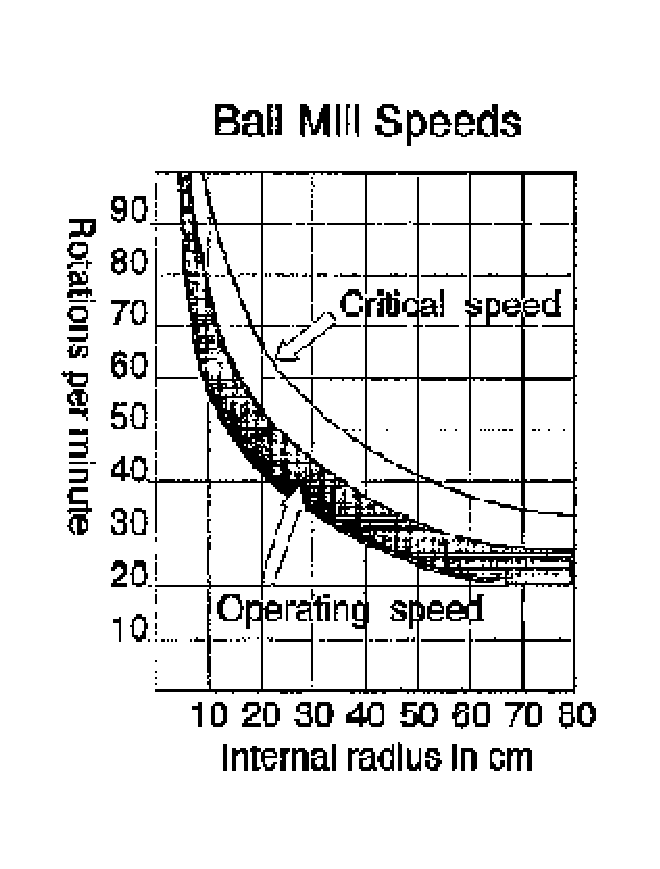
\includegraphics[width=0.8\linewidth]{img/ballmillspeed.eps}
  \caption{Graph of ball mill speeds.}
  \label{fig:ballmillspeed}
\end{figure}
%-------------------------------------------------------------------------------
\begin{figure}[htbp!]
  \centering
  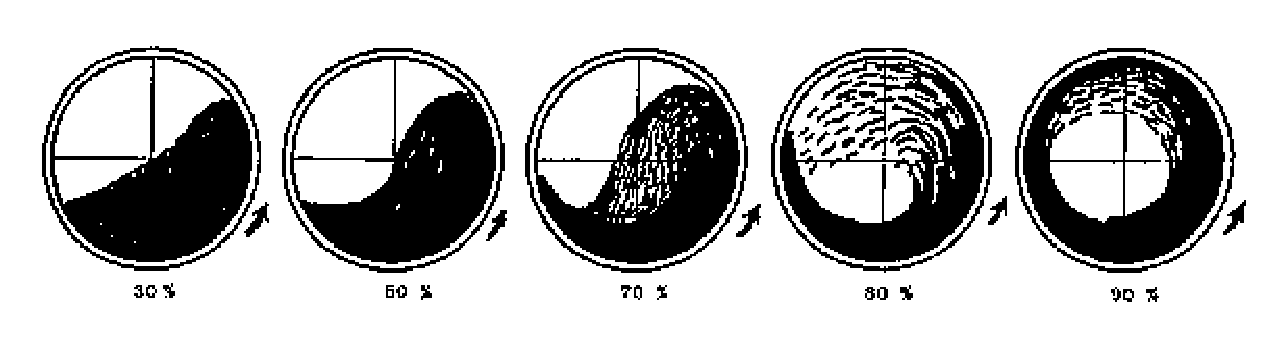
\includegraphics[width=0.8\linewidth]{img/ballmillefficient.eps}
  \caption{A cross section of a ball mill running at speeds from 30-90\% of 
  critical speed. At 30\% the grinding takes place mainly between pebbles and 
  lining, at 70\% a good cascading rolling produces efficient grinding, and at 
  90\% very little grinding takes place.}
  \label{fig:ballmillefficient}
\end{figure}
%-------------------------------------------------------------------------------
\subsubsection{Charge}
Table~\ref{tab:charge} shows the charge for a ball mill (by volume), with a 
speed of 60--80\% of critical speed.

When the mill is filled to maximum capacity, the speed should be closer to 60\% 
of critical speed. The water content should be enough to produce a thin slip. 
After filling, about 30\% of the volume should remain empty. If you measure all 
the materials separately, total volume may seem to be 85\% of ball mill 
capacity. However, since the water and material fill the spaces between the 
balls, this will still result in 30\% empty space.
%------------------------------------------------------------------------------
\begin{center}
          \renewcommand{\arraystretch}{1.5}
  \begin{table}\centering
    \begin{tabular}{|c|c|}\hline
      \textbf{Ingredient}&\textbf{Percent}\\\hline\hline
      %------------------------------------------------------------------------------
      Pebbles&45--55\%\\\hline
      %------------------------------------------------------------------------------
      Water&12--20\%\\\hline
      %------------------------------------------------------------------------------
      Material&20--25\%\\\hline
    \end{tabular}
    \caption{Proportions of charge in a ball mill at 60--80\% of critical 
      speed.}
    \label{tab:charge}
  \end{table}
\end{center}
%------------------------------------------------------------------------------
\subsubsection{Example}
A ball mill with new lining measures inside:

Width = $0.64 m$ 
Diameter = $0.445 m$

volume~of~ball~mill = $pi * r^2 * w$ (= \textbf{320 liters})

critical~speed = $29.9 / \sqrt{r}$ (= \textbf{58.2 RPM})

60--80\% of the critical speed = 31.7 RPM--42.3 RPM

A typical glaze has a density (specific gravity) of approximately 2.7. That 
means that the glaze charge should be 24-30 kg. For a breakdown of the charge, 
see table~\ref{tab:chargeexample}
%------------------------------------------------------------------------------
\begin{center}
          \renewcommand{\arraystretch}{1.5}
  \begin{table}\centering
    \begin{tabular}{|c|c|}\hline
      \textbf{Ingredient}&\textbf{Percent}\\\hline\hline
      %------------------------------------------------------------------------------
      Pebbles&144--176 liters\\\hline
      %------------------------------------------------------------------------------
      Water&38--64 liters\\\hline
      %------------------------------------------------------------------------------
      Material&64--80 liters\\\hline
    \end{tabular}
    \caption{Charge (by volume) of the example ball mill.}
    \label{tab:chargeexample}
  \end{table}
\end{center}
%------------------------------------------------------------------------------
\subsubsection{Ball Milling Time}
The time for ball milling varies with the hardness of materials. Soft materials 
such as frits may require only 2-3 hours, whereas hard materials like quartz 
can take 24 hours or more.

When you ball-mill standard materials, it is important to mill each batch for 
the same amount of time. For this reason, it is a wise investment to purchase a 
timer switch for the mill. This will avoid human errors. Too much ball milling 
can cause glaze crawling.
%------------------------------------------------------------------------------
\subsubsection{Operating Procedure}
Before each operation:
%------------------------------------------------------------------------------
\begin{itemize}
\item Check that the ball mill is clean inside.
\item Check that pebbles fill half of the ball mill -refill if necessary.
\item Fill in materials (20-25\% of mill volume).
\item Fill water until pebbles and material are just covered.
\item Be very careful about correct ball milling time. If possible, use an 
automatic timer.
\end{itemize}
%------------------------------------------------------------------------------
After operation:
%------------------------------------------------------------------------------
\begin{itemize}
\item After emptying the ball mill, clean it thoroughly with water by filling 
it and running it with the pebbles. If the same material is to be ground, 
cleaning is not needed.
\end{itemize}
Every month:
%------------------------------------------------------------------------------
\begin{itemize}
\item Empty the pebbles out and remove all pebbles that are too flat or less 
than 2 cm in diameter.
\item Inspect the inside lining for signs of wear, and repair as necessary.
\end{itemize}
%------------------------------------------------------------------------------
\section{Weighing, Mixing, Using Batch Cards}
\subsection{Weighing Glaze Ingredients}
First, you must have an accurate scale. This can be a small balance, such as is 
used by jewelers, or a triple beam balance, which is faster to use. Spring 
scales are not accurate enough, nor are postal scales. For large quantities, 
the most accurate low-cost balance is the common beam balance which uses 
standard weights.
%-------------------------------------------------------------------------------
\begin{figure}[htbp!]
  \centering
  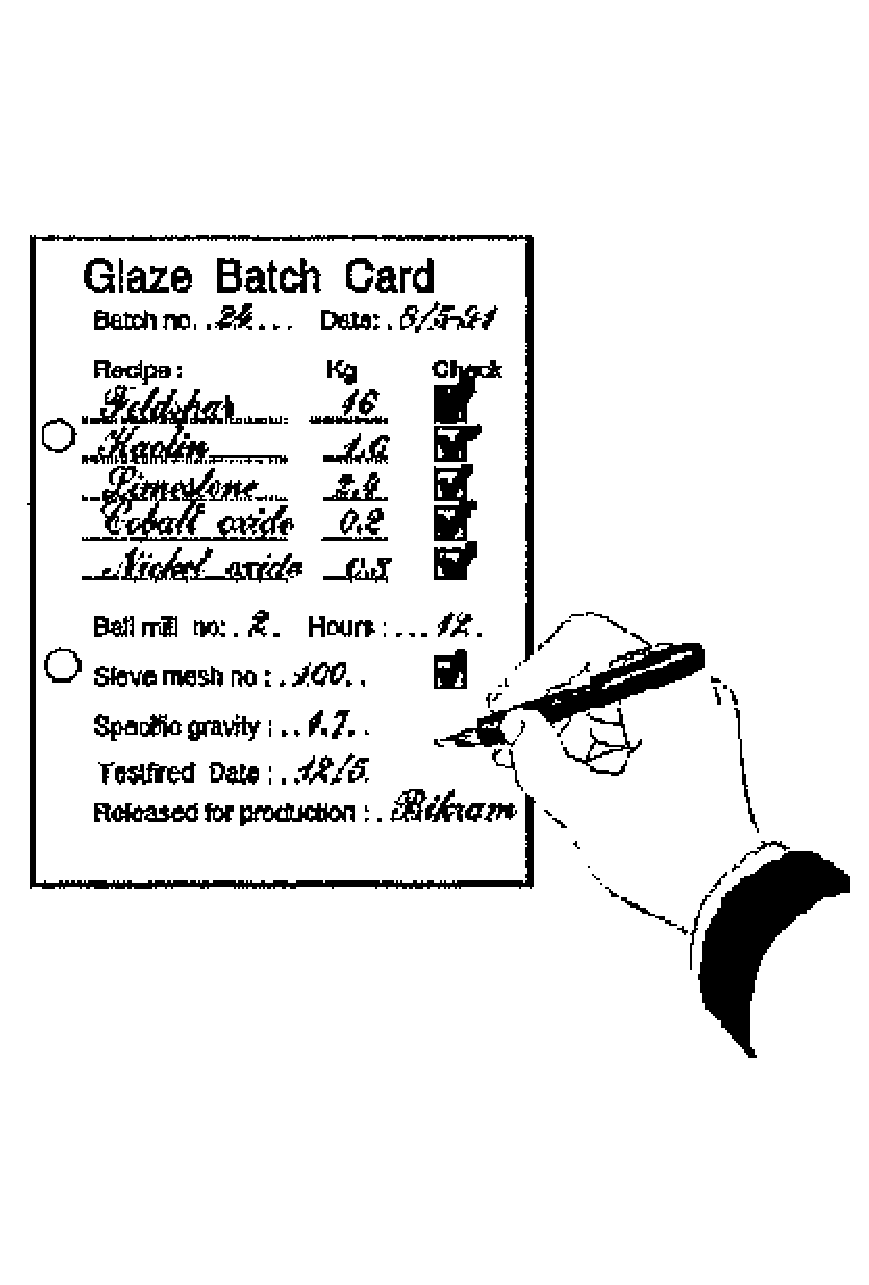
\includegraphics[width=0.8\linewidth]{img/batchcard.eps}
  \caption{Example of a glaze batch card used for qualitz control.}
  \label{fig:batchcard}
\end{figure}
%-------------------------------------------------------------------------------
\subsection{Batch Cards}
\label{sec:batchcard}
For best results, a batch card system should be used. These are simply cards 
that have the glaze recipe written on them. As each ingredient is weighed, it 
is checked off on the list. When all materials are weighed, the batch card is 
given a number (usually the date). The same number is written on the glaze 
container. This makes it easier to find out the problem when the glaze does not 
work correctly.
%------------------------------------------------------------------------------
\subsection{Water}
The ingredients are then added to a container which already has the approximate 
amount of water in it. 

\textbf{CAUTION:} The water must always be clean. After mixing, the water is 
adjusted. It is always best to start with less water than required. If the 
glaze is too fluid, it is difficult to remove excess water.
%------------------------------------------------------------------------------
\subsection{Containers}
Glazes are normally sieved through a 100-mesh screen. The glaze should be 
poured through without forcing it. Never use your hand to force glaze through a 
sieve, as this will quickly break down the wire mesh. A brush should be used 
instead.
%------------------------------------------------------------------------------
\section{Sieving}
Glazes are normally sieved through a 100-mesh screen. The glaze should be 
poured through without forcing it. Never use your hand to force glaze through a 
sieve, as this will quickly break down the wire mesh. A brush should be used 
instead.
%------------------------------------------------------------------------------
\section{Suspending and Binding Agents}
Because glazes are mixtures and not solutions, they tend to settle at the 
bottom of the container. Normally, the clay content of the glaze will be 
sufficient to keep them in suspension during application. However, some glazes 
tend to settle as a cement-like layer on the bottom and are difficult to stir. 
These glazes require the addition of a suspending agent.
%------------------------------------------------------------------------------
\subsection{Suspending Agent}
The most common suspending agent is bentonite, in 1-2\% additions. This will 
normally not be enough to affect the glaze when fired. Dry bentonite cannot be 
added to wet glaze, as it will just form lumps and be impossible to mix in 
thoroughly. Instead it should either be mixed separately with water into a thin 
slip and then added to the glaze or it should be added to the dry glaze and 
mixed in well before adding water.
%------------------------------------------------------------------------------
\subsection{Binder}
Another common problem is that some glazes tend to be powdery, and come off 
when loading the kiln. For this problem a binder is added.

Bentonite also works as a binder and is the simplest to use. Another common 
binder is CMC gum (carboxymethyl cellulose), which is available in either 
liquid or powder form. The liquid can be used directly, about 1\%. The powder 
needs to be dissolved in water (1:10) overnight and then is added to the glaze 
as liquid.

Organic binders such as gum arable, wheat flour, sugar or starch (0.1--0.5\% of 
dry glaze) are sometimes used. These have the disadvantage of fermenting. They 
should be used immediately after mixing, or if stored a few drops of chlorine 
bleach or formaldehyde can be added as a preservative.

Addition of 1\% raw borax produces a hard surface that does not powder when 
painted on.
%------------------------------------------------------------------------------
\subsection{Flocculation}
Addition of a flocculation agent will make the glaze more creamy. The pottery 
will absorb the water more easily so glaze is picked up faster.

This works better in combination with clay or bentonite. Common flocculants 
are: Epsom salts (magnesium sulfate), calcium chloride, calcium nitrate and 
borax. They are prepared by adding 100 g flocculant to 200 ml hot water and the 
solution is added to the glaze one tablespoonful at a time (up to 1\% of dry 
glaze weight). Plaster of parts (already set) can also be used.

Flocculation is also used for nonporous ware often in combination with a 
binder. The creamy glaze forms a thick loose layer that stays on the nonporous 
surface.
%------------------------------------------------------------------------------
\subsection{Deflocculation}
When the glaze is deflocculated it becomes more fluid with the same amount of 
water. This is sometimes used for glazing nonporous ware that cannot absorb 
water. Sodium silicate and soda ash are the most common deflocculants and they 
are prepared in the same way as flocculants.

\textbf{CAUTION:} Binders, deflocculants or flocculants should only be added 
after the glaze is ball-milled.
%------------------------------------------------------------------------------
\section{Density and Specific Gravity}
Most potters judge the consistency of their glaze by experience and feel, or by 
test application to a few pieces of biscuit to see if the thickness is correct. 
The standard test is to check thickness with a fingernail, which is a very 
accurate test for an experienced glazer. Then adjust the water as necessary.

A more accurate method is to measure the specific gravity of the glaze with a 
hydrometer, such as is commonly used to judge the amount of water that has been 
mixed with milk. When reading the depth the hydrometer sinks, take care that it 
is really showing the correct density. If the glaze is thick you have to 
vibrate the bucket repeatedly to make sure the hydrometer sinks in.

Specific gravity (s.g.) is a measure of the density of a liquid compared to 
water, which has a standard specific gravity of 1. Glazes will always be 
heavier than water. The specific gravity is found by weighing a specific 
volume, say 1000 ml (milliliters). If this weighs 1500 g the s.g. is 1.5. 
Weighing is more accurate than using a hydrometer.

After you find out the correct amount of water by trial and error, the specific 
gravity can be measured and future batches of the same glaze made to the same 
specific gravity.

\textbf{CAUTION:} This is not always a reliable method because the water 
absorption of your biscuit will vary with its firing temperature. The water 
will still need to be adjusted by trial and error. Trial application and 
testing with a fingernail still constitute the most reliable method.
%-------------------------------------------------------------------------------
\begin{figure}[htbp!]
  \centering
  \includegraphics[width=0.8\linewidth]{img/Hydrometer.eps}
  \caption{Hydrometer made from a glass test tube..}
  \label{fig:Hydrometer}
\end{figure}
%-------------------------------------------------------------------------------
\section{Old Glazes, and Problems}
If you keep wet glazes around for a long time, they will usually have problems 
with settling or drying up. These glazes can still be used but it will be 
necessary to adjust the water and to resieve them. If the glaze is extremely 
thick, it is sometimes best to dry it out completely, crush it and remix it.

Before using a glaze that has set in the bucket for a few days, it should 
always be sieved through 60 or 100 mesh.

Too much water in the glaze is also a problem. The glaze can be allowed to 
settle and excess water carefully taken off the top. 

\textbf{CAUTION:} With soluble glazes, this can remove some of the ingredients 
and result in a glaze that no longer works correctly. In this case, the water 
should be allowed to evaporate until the thickness is correct.

Glazes made with raw borax, or incomplete borax frits, will often grow 
crystals. These cannot be sieved. The glaze should be dried out, the crystals 
crushed and remixed.

Some glazes will develop mold and begin to smell. Although they can still be 
used, it is probably better to just throw them out.
%-------------------------------------------------------------------------------
\section{Test Your Glazes}
The wise potter will never glaze a kilnload with untested glaze. Enough glaze 
should be kept on hand, so that each new batch can be test-fired in the regular 
glaze firing before it is used for application.
%-------------------------------------------------------------------------------
\section{Commercial Production of Glazes}
Glazes that are sold commercially are usually in dry powder form. They are made 
as standard glazes by ball milling, then are dried and packaged.

These glazes are simply mixed with the correct amount of water and sieved 
before using.
%-------------------------------------------------------------------------------